\section{Methods (The Structure of a Paper)}
\label{sec:methods}
\label{sec:structure-paper}



\subsection{Dictionary learning}

Another direction in which we investigated is the construction of the dictionary we would use for our sparse coding. The nature of a dictionary not only determines the quality of the inpainting result, but also the speed of the inpainting process, depending on the size of the dictionary as well as the degree of sparseness reachable with it. 
The choice of dictionary was particularly of interest in our case to improve the running time. The approach we adopted for the reconstruction of the image would a priori assure a good quality of the reconstruction, however on the expense of the time necessary for the reconstruction, hence the need of a dictionary which would limit this trade-off without affecting too much the improved quality of the reconstruction.
With this objective in mind, we built a under-complete dictionary on the space of patches of size 16x16, composed of 64 atoms (25 percent of the total dimension), by applying the approximate K-SVD algorithm on a training data customized for our need. We also paid particular attention to the initialization of the learning process, since this method is known to be initialization-sensitive [TODO REF]. In the rest of this section we will refer to the space of patches of size 16x16 as $E$.

\mypar{K-SVD algorithm}
The algorithm takes a training set of patches $X$, and learn a dictionary $U$, starting from an initialized value of $U$ and iteratively learning to fit to $X$ in a more efficient way. 
For all dictionaries, we used this algorithm with 15 iterations, using the same training data set.

\mypar{Training Data set}
The dictionary being under-complete, loss of information will inevitably occur. The atoms will hence need to be very efficient in reconstructing the image without losing important information. In other words, the atoms need to be able to describe characteristics of patches that have a high-variability among the kind of patches that we want to reconstruct. The aspects of patches with low-variability can be easily estimated by the mean, with a minimal loss of information. 
To achieve this, we first gathered patches of size 16x16 extracted from 36 pictures of size 512x512, consisting of photography of cities, nature and animals. We then applied principal component analysis (PCA) on these patches to deduce the most significant subspace of $E$ of dimension 64, i.e. the subspace of $E$ that include the highest variability of value among patches of real-world photography. We then projected the whole training set as well as our learning process onto that subspace. That way, we ensure that the learned 64 atoms stay in this a priori significant subspace, without getting lost into the less-meaningful directions of $E$, allowing them to efficiently reconstruct a patch.

\mypar{Initialization}
The algorithm we chose is sensitive to the choice of the initial candidate, it optimizes it locally and greedily until no progress is possible. We implemented 2 main different ways to initialize the learning process:
\begin{itemize}
   \item From a known dictionary: in this method, we initialize the dictionary on a known dictionary, such as a 64-atom DCT (Discrete Cosine Transform) dictionary, or the 64 significant vectors obtained by applying PCA to the training set.  
   \item k-means initialization: in this method, we initialize the dictionary based on the training data set. We first center and normalize the training data, after which we apply the K-means algorithm with K=64 based on the euclidean norm, and use the normalized 64 centroids as initializing atoms. To improve the robustness of the K-mean algorithm, we applied the algorithm 10 times and chose the result which had the smallest mean pairwise-distance with other clustering. 
\end{itemize}
A randomly-generated atom initialization have also been implemented to serve as a reference for studying the efficiency of other initialization methods. 

Lastly, to compare the efficiency of the overall dictionary performance, we set the baseline reference as the standard complete DCT dictionary.

































TODO: Subsection ``Background" to introduce roughly the concepts of sparse coding.

TOOD: Present our method.

TODO: Present baseline method and Criminisi method. (My suggestion is to compare the results of our algorithm with the class winner. They probably will like this approach. We probably won't beat the performance of the Criminisi approach in general, but we might be better in some cases, furthermore we will be faster for sure...

Scientific papers usually begin with the description of the problem,
justifying why the problem is interesting. Most importantly, it argues
that the problem is still unsolved, or that the current solutions are
unsatisfactory. This leads to the main gist of the paper, which is
``the idea''. The authors then show evidence, using derivations or
experiments, that the idea works. Since science does not occur in a
vacuum, a proper comparison to the current state of the art is often
part of the results. Following these ideas, papers usually have the
following structure:
\begin{description}
\item[Abstract] \ \\
  Short description of the whole paper, to help the
  reader decide whether to read it.
\item[Introduction] \ \\
  Describe your problem and state your
  contributions.
\item[Models and Methods] \ \\
  Describe your idea and how it was implemented to solve
  the problem. Survey the related work, giving credit where credit is
  due.
\item[Results] \ \\
  Show evidence to support your claims made in the
  introduction.
\item[Discussion] \ \\
  Discuss the strengths and weaknesses of your
  approach, based on the results. Point out the implications of your
  novel idea on the application concerned.
\item[Summary] \ \\
  Summarize your contributions in light of the new
  results.
\end{description}


\section{Tips for Good Writing}
\label{sec:tips-writing}

The ideas for good writing have come
from~\cite{editor10,jones08,anderson04}.

\subsection{Getting Help}
One should try to get a draft read by as many friendly people as
possible. And remember to treat your test readers with respect. If
they are unable to understand something in your paper, then it is
highly likely that your reviewers will not understand it
either. Therefore, do not be defensive about the criticisms you get,
but use it as an opportunity to improve the paper. Before your submit
your friends to the pain of reading your draft, please \emph{use a
  spell checker}.

\subsection{Abstract}
The abstract should really be written last, along with the title of
the paper. The four points that should be covered~\cite{jones08}:
\begin{enumerate}
\item State the problem.
\item Say why it is an interesting problem.
\item Say what your solution achieves.
\item Say what follows from your solution.
\end{enumerate}

\subsection{Figures and Tables}

\begin{figure}[tbp]
  \centering
  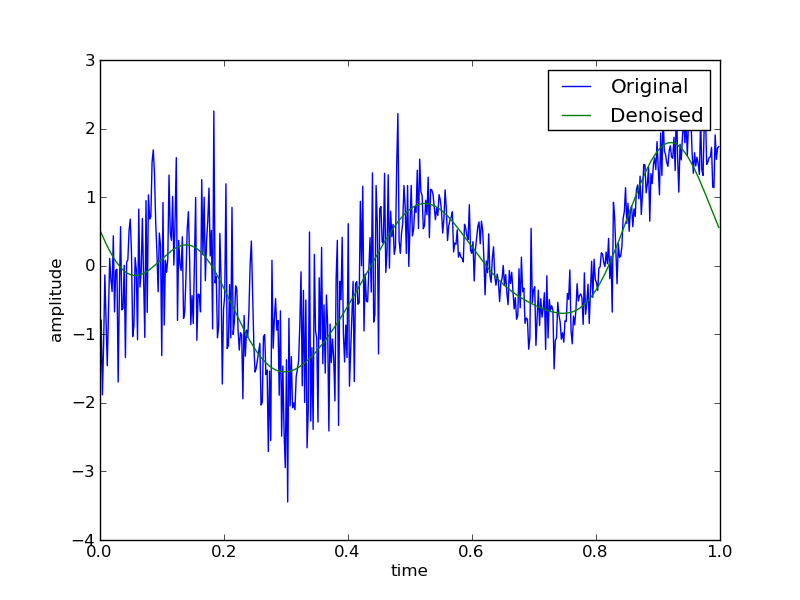
\includegraphics[width=\columnwidth]{graphics/denoised_signal_1d}
  \caption{Signal compression and denoising using the Fourier basis.}
  \label{fig:denoise-fourier}
\end{figure}
\begin{figure}[htbp]
  \centering
  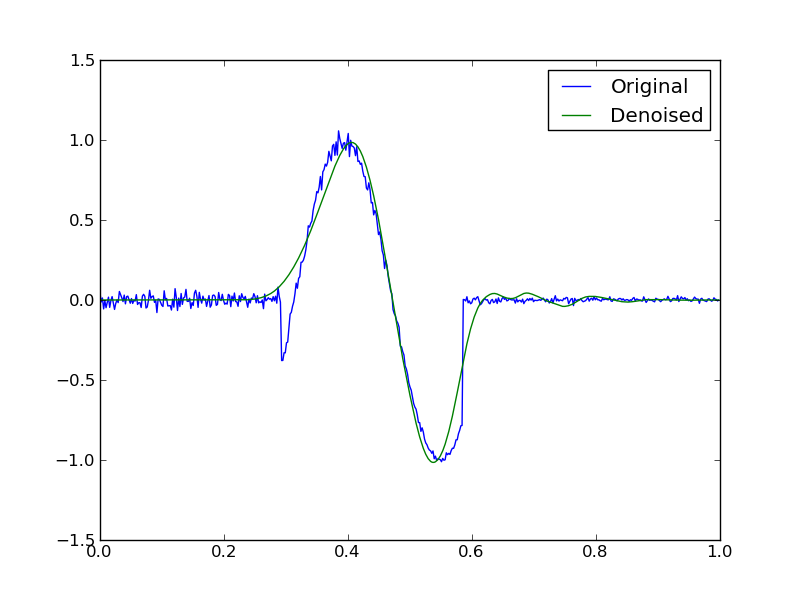
\includegraphics[width=\columnwidth]{graphics/local_wdenoised_1d}
  \caption{Signal compression and denoising using the Daubechies wavelet basis.}
  \label{fig:denoise-wavelet}
\end{figure}

Use examples and illustrations to clarify ideas and results. For
example, by comparing Figure~\ref{fig:denoise-fourier} and
Figure~\ref{fig:denoise-wavelet}, we can see the two different
situations where Fourier and wavelet basis perform well. 

\subsection{Models and Methods}
The models and methods
section should describe what was
done to answer the research question, describe how it was done,
justify the experimental design, and
explain how the results were analyzed.

The model refers to the underlying mathematical model or structure which 
you use to describe your problem, or that your solution is based on. 
The methods on the other hand, are the algorithms used to solve the problem. 
In some cases, the suggested method directly solves the problem, without having it 
stated in terms of an underlying model. Generally though it is a better practice to have 
the model figured out and stated clearly, rather than presenting a method without specifying 
the model. In this case, the method can be more easily evaluated in the task of fitting 
the given data to the underlying model.

The methods part of this section, is not a step-by-step, directive,
protocol as you might see in your lab manual, but detailed enough such
that an interested reader can reproduce your
work~\cite{anderson04,wavelab}.

The methods section of a research paper provides the information by
which a study's validity is judged.
Therefore, it requires a clear and precise description of how an
experiment was done, and the rationale
for why specific experimental procedures were chosen.
It is usually helpful to
structure the methods section by~\cite{kallet04methods}:
\begin{enumerate}
\item Layout the model you used to describe the problem or the solution.
\item Describing the algorithms used in the study, briefly including
  details such as hyperparameter values (e.g. thresholds), and
  preprocessing steps (e.g. normalizing the data to have mean value of
  zero).
\item Explaining how the materials were prepared, for example the
  images used and their resolution.
\item Describing the research protocol, for example which examples
  were used for estimating the parameters (training) and which were
  used for computing performance.
\item Explaining how measurements were made and what
  calculations were performed. Do not reproduce the full source code in
  the paper, but explain the key steps.
\end{enumerate}

\subsection{Results}

Organize the results section based on the sequence of table and
figures you include. Prepare the tables and figures as soon as all
the data are analyzed and arrange them in the sequence that best
presents your findings in a logical way. A good strategy is to note,
on a draft of each table or figure, the one or two key results you
want to address in the text portion of the results.
The information from the figures is
summarized in Table~\ref{tab:fourier-wavelet}.

\begin{table*}[htbp]
  \centering
  \begin{tabular}[c]{|l||l|l|l|}
    \hline
    Basis&Support&Suitable signals&Unsuitable signals\\
    \hline
    Fourier&global&sine like&localized\\
    wavelet&local&localized&sine like\\
    \hline
  \end{tabular}
  \caption{Characteristics of Fourier and wavelet basis.}
  \label{tab:fourier-wavelet}
\end{table*}

When reporting computational or measurement results, always
report the mean (average value) along with a measure of variability
(standard deviation(s) or standard error of the mean).
